\chapter{Infraestructura}\label{cap.infraestructura}
En este capítulo se expondrán los principales componentes software utilizados, centrados, principalmente, en la conexión con la cámara y el desarrollo, entrenamiento y test de la red neuronal. Además, se expone una descripción de las bases de datos de las que se partirá para realizar las distintas pruebas sobre la red neuronal. Estas bases de datos serán luego modificadas y adaptadas para el problema concreto que se plantee, permitiendo obtener diversas conclusiones acerca del comportamiento de la propia red y, así, emplear la más adecuada.\\
\section{Software}
\subsection{JdeRobot}
JdeRobot \footnote{http://jderobot.org} es una plataforma de software libre que facilita la tarea de los desarrolladores del campo de la robótica, visión por computador y otras relacionadas, siendo este su principal fin.\\ 

Está escrito en su mayoría en el lenguaje C ++ y proporciona un entorno de programación basado en componentes distribuidas, de tal manera que una aplicación está formada por una colección de varios componentes asincrónos y concurrentes. Esta estructura permite la ejecución de los distintos componentes en diferentes equipos, estableciendo una conexión entre ellos mediante el middleware de comunicaciones ICE. Además, se obtiene gran flexibiidad a la hora de desarrollar las aplicaciones, ya que estos componentes pueden escribirse en C ++, Python, Java ... y todos ellos interactúan a través de interfaces ICE explícitas.\\ 

A pesar de que esta plataforma incluye una gran variedad de herramientas y librerías para la programación de robots, y de una amplia gama de componentes previamente desarrollados para realizar tareas comunes en este ámbito, no es la verdadera finalidad del proyecto su uso, por lo que únicamente se centrará en la utilización de uno de sus componentes para facilitar la obtención de las imágenes.\\

\begin{description}
\item[Camera Server] \hfill 
\vspace{10pt}
\\
Se trata de un componente que permite servir a un número determinado de cámaras, ya sean reales o simuladas a partir de un archivo de vídeo. Internamente gstreamer para el manejo y el procesamiento de las diferentes fuentes de vídeo.\\
\vspace{-10pt}
\\
Para su uso, es necesario editar su fichero de configuración, adaptándolo a las necesidades concretas que plantee la máquina. Dentro de este fichero se permite especificar los siguientes campos:\\
\vspace{-20pt}
\begin{itemize}
    \item Configuración de la red, donde se indica la dirección del servidor que va a recibir la petición.
    \item Número de cámaras que se servirán.
    \item Configuración de las cámaras. Se podrán modificar los siguientes campos para cada cámara:
    \begin{itemize}
         \item Nombre y breve descripción
         \item URI: string que define la fuente de vídeo
     	 \item Numerador y denominador del frame rate
         \item Altura y anchura de la imagen
         \item Formato de la imagen
         \item Invertir o no la imagen 
    \end{itemize}
\end{itemize}
\end{description}

\subsection{Caffe}
Caffe \footnote{http://caffe.berkeleyvision.org/} es un framework de deep learnirng que permite el desarrollo, entrenamiento y evaluación de redes neuronales. Incluye, además, modelos y ejemplos previamente trabajados para un mejor entendimiento de las redes neuronales. Es una plataforma de software libre, escrito en C ++ ,  que utiliza la librería CUDA para el aprendizaje profundo y permite interfaces escritas en Python o Matlab.\\ 

Esta plataforma es interesante por múltiples factores. Además de incluir múltiples ejemplos y modelos ya entrenados, lo que ofrece mayor agilidad a la hora de empezar a entender el funcionamiento del aprendizaje profundo, es destacabla la velocidad que ésta ofrece para el entrenamiento de las redes y su posterior evaluación, ya que está prevista con varios indicadores que permiten evaluar la propia red y compararla con otras.\\ 

Su base se encuentra en las redes neuronales convolucionales explicadas en el Capítulo \ref{}, utilizando un entrenamiento por lotes. En concreto, su estructura y funcionamiento básico queda explicado en la Figura~\ref{fig.redCaffe}, donde se .\\

\begin{figure}[h!]
	\begin{center}
		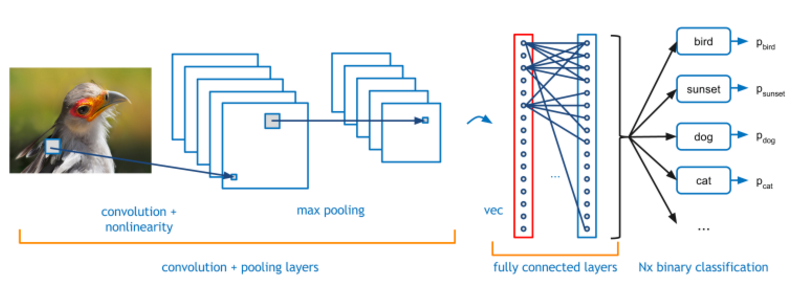
\includegraphics[width=0.6\textwidth]{figures/red_caffe}
		\caption{Estructura y funcionamiento básico de red en Caffe}
		\label{fig.redCaffe}
	\end{center}
\end{figure}

La plataforma utiliza una serie de capas (\textit{layers}), que, según su configuración y la distinta conexión entre ellas, permite la creación de diferentes redes neuronales. Estas etiquetas se dividen en varios grupos, en función del tipo de entrada, el tipo de salida o la función que realiza cada una de ellas. Este trabajo no utiliza todas las capas existentes en la plataforma, a continuación se explicarán cada una de las capas empleadas, clasificadas según al grupo que pertenecen.\\
\vspace{-20pt}

\begin{description}
\item[Data Layers] \hfill 
\vspace{10pt}
\\
	Su uso se centra en la introducción de datos a la red neuronal, y estarán situadas siempre en la parte inferior de la misma. Estos datos pueden provenir de diferentes vías como bases de datos eficientes como LMDB, utilizada en este trabajo, diréctamente desde la memoria o desde archivos en disco en HDF5 o formatos de imagen comunes.\\
	Dentro de esta capa es posible, además de especificar la ruta de los datos y el tamaño del lote (\textit{batch}), indicar la fase en la que se utilizarán los datos, entrenamiento o test, así como algunos parámetros de transformación para el preprocesamiento de la imagen. En concreto, en este trabajo, se utilizarán datos de entrada para ambas fases y un factor de escala para establecer el rango de las imágenes en [0,1].
	\vspace{15pt}
	
\item[Vision Layers] \hfill 
\vspace{10pt}
\\
	Típicamente toman una imagen de entrada y producen otra de salida, de forma que, aplicando una operación particular a alguna región de la entrada, se obtiene la región correspondiente de la salida. Caffe dispone de varias capas de este estilo, a continuación se comentan las dos utilizadas en el trabajo.
	\vspace{10pt}
	\begin{description}
	\item[Convolution Layer] \hfill 
	\vspace{5pt}
	\\
		Realiza la convolución de la imagen de entrada con un conjunto de filtros de aprendizaje, cada uno produciendo un mapa de características en la imagen de salida. Se deben especificar datos como el número de salidas, el tamaño del filtro, el desplazamiento entre cada paso del filtro, y la inicialización y relleno de los pesos y bias.
		\vspace{10pt}
	\item[Pooling Layer] \hfill 
	\vspace{5pt}
	\\
		Combina la imagen de entrada tomando el máximo, el promedio, u otras operaciones dentro de las regiones, siendo su finalidad la reducción del muestreo. En esta capa se pueden especificar parámetros como el tipo de pooling a realizar, máximo, promedio o estocástico, el tamaño del filtro o el desplazamiento entre cada paso del filtro.
	\end{description}

\vspace{70pt}
\item[Common Layers] \hfill
	\begin{description}
	\item[Inner Product] \hfill 
	\vspace{5pt}
	\\
	Calcula un producto escalar con un conjunto de pesos aprendidos, y, de manera opcional, añade sesgos. Trata la entrada como un simple vector y produce una salida en forma de otro, estableciendo la altura y el ancho de cada \textit{bolb} en 1. Se establece el número de salidas, y la inicialización y relleno de los pesos y bias.
	\vspace{10pt}
	\item[Dropout] \hfill 
	\vspace{5pt}
	\\
	Durante el entrenamiento, únicamente, establece una porción aleatoria del conjunto de entrada a 0, ajustando el resto de la magnitud del vector en consecuencia, evistando así el sobre ajuste. Se debe indicar el ration en un valor del 0 a 1, que indicará el porcentaje de muestras que se ignorarán.
	\end{description}

\vspace{15pt}	
\item[Activation / Neuron Layers] \hfill  
\vspace{10pt}
\\
	En general, estas capas, son operadores de elementos, que toman un \textit{bolb} inferior y producen uno superior del mismo tamaño. Existen varias capas con este funcionamiento en la plataforma, en concreto se empleará la ReLu.
	\vspace{10pt}
	\begin{description}
	\item[ReLu] \hfill  
	\vspace{5pt}
	\\
		Utiliza la función $y=max(0,x)$ cuya gráfica se define en la Figura~\ref{fig.reLu}
		\begin{figure}[h!]
			\begin{center}
				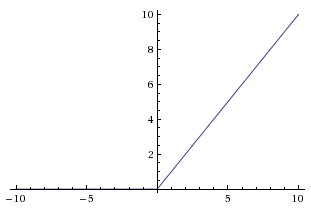
\includegraphics[width=0.5\textwidth]{figures/relu.jpeg}
				\caption{Función de activación ReLu}
				\label{fig.reLu}
			\end{center}
		\end{figure} 
	\end{description}
	
\vspace{50pt}
\item[Loss Layers] \hfill 
\vspace{10pt}
\\
	El cálculo de la pérdida permite el aprendizaje mediante la comparación de la salida con un objetivo y la asignación de un coste para minimizarla. Se calcula mediante el paso hacia adelante. Existen diferentes medidas de las que se destacan dos.
	\vspace{10pt}
	\begin{description}
	\item[Softmax with Loss] \hfill 
	\vspace{5pt}
	\\
		Se calcula como: 
		$$E = \frac{-1}{N} \sum\limits_{n=1}^N \log(\hat{p}_{n,l_n})$$
		Siendo $N$ el número total de muestras y $\hat{p}$ las probabilidades de cada etiqueta para cada muestra.
		\vspace{10pt}
	\item[Accuracy] \hfill 
	\vspace{5pt}
	\\
		Se calcula como:
		$$\frac{1}{N} \sum\limits_{n=1}^N \delta\{ \hat{l}_n = l_n \}$$
		donde $\delta\{ \textup{condición}\} = \left\{ \begin{array}{lr} 1 &  \textup{si condición} \\ 0 & \mbox{resto} \end{array} \right.$
	\end{description}
	
\end{description}
\vspace{20pt}
Por último, además de las capas y parámetros definidos anteriormente, Caffe, permite el desarrollo de un \textit{solver} en el que se podrán ajustar parámetros como el número de iteraciones totales que se ejecutarán, el de test que se van a realizar, cada cuantas iteraciones se realizarán esos test, así como se sacarán redes intermedias.\\
Para Caffe, el número de iteraciones no se corresponde con el número de veces que la red recorre la base de datos al completo, sino como las veces que se pasa por cada lote al completo. De esta manera, se define el número de épocas, es decir, el número de veces que se recorre de manera completa la base de datos, con la siguiente expresión:\\
$$\textup{N.Epocas}=\frac{\textup{Tamaño lote de entrenamiento}\times \textup{Total iteraciones}}{\textup{Muestras entrenamiento}} $$\\
En cuanto al número de iteraciones que se establecerán de test, se debe cumplir la siguiente igualdad:
$$\textup{Iteraciones test}=\frac{\textup{Muestras test}}{\textup{Tamaño lote de test}}$$

\section{Bases de datos}
\subsection{MNIST}
MNIST \footnote{http://yann.lecun.com/exdb/mnist/} está formada por diferentes imágenes con números escritos a mano y consta de un conjunto de entrenamiento de 60.000 ejemplos y otro de prueba de 10.000 ejemplos. Es una buena base de datos para personas que quieren probar técnicas de aprendizaje y métodos de reconocimiento de patrones en datos del mundo real, mientras que dedican un mínimo esfuerzo a preprocesar y formatear. \\

Se trata de un subconjunto de una más grande, NIST, en la que las imágenes originales en blanco y negro (NIV) fueron normalizadas en el tamaño para encajar en un cuadro de 20x20 píxeles, preservando su relación de aspecto. Las imágenes obtenidas contienen niveles de gris como resultado de la técnica anti-aliasing utilizada por el algoritmo de normalización. Estas imágenes se centraron en una de 28x28 calculando el centro de masa de los píxeles y trasladando la imagen para situar este punto en el centro del campo 28x28.\\

Fue construida a partir de la Base de Datos Especial 3 y la Base de Datos Especial 1 del NIST, que contienen imágenes binarias de dígitos manuscritos. NIST originalmente designó SD-3 como su conjunto de entrenamiento y SD-1 como su conjunto de pruebas. Sin embargo, SD-3 es mucho más limpio y más fácil de reconocer que SD-1.Esto es debido a que SD-3 fue recogido entre los empleados de la Oficina del Censo, mientras que el SD-1 fue recogido entre los estudiantes de secundaria. Dado que para una buena extracción de conclusiones es necesario que el resultado sea independiente de la elección del conjunto de entrenamiento y de prueba entre el conjunto completo de muestras, fue necesaria la elaboración de un nuevo conjunto en el que ambas bases de datos estuviesen representadas de manera equitativa. Además, se aseguraron de que los conjuntos de escritores en el de entrenamiento y el de prueba son disjuntos.

\subsection{COCO}
Microsoft COCO \footnote{http://mscoco.org/} es un gran conjunto de datos de imágenes diseñado para la detección de objetos, segmentación y generación de subtítulos. Alguna de las características principales de este conjunto de datos son:
	\begin{itemize}
         \item Múltiples objetos en cada imagen
     	 \item Más de 300.000 imágenes
         \item Más de 2 millones de instancias
         \item 80 categorías de objetos
    \end{itemize}
    
Esta plataforma se ha desarrollado para varios retos, en concreto es de interés el reto de la detección, establecido en 2016. Se utilizan conjuntos de entrenamiento, prueba y validación con sus correspondientes anotaciones. COCO tiene tres tipos de anotaciones: instancias de objeto, puntos clave de objeto y leyendas de imagen, que se almacenan utilizando el formato de archivo JSON y comparten estructura de datos establecida en la Figura~\ref{fig.basicStruc}. \\

Para la detección son de interés las anotaciones de instancias de objetos, cuya estructura se muestra en la Figura~\ref{fig.objInst}.Cada anotación de instancia contiene una serie de campos, incluyendo el ID de categoría y la máscara de segmentación del objeto. El formato de segmentación depende de si la instancia representa un único objeto (iscrowd = 0), en cuyo caso se utilizan polígonos, o una colección de objetos (iscrowd = 1), en cuyo caso se utiliza RLE. Debe tenerse en cuenta que un único objeto puede requerir múltiples polígonos, y que las anotaciones de la multitud se utilizan para etiquetar grandes grupos de objetos. Además, se proporciona una caja delimitadora para cada objeto, cuyas coordenadas se miden desde la esquina superior izquierda de la imagen y están indexadas en 0. Finalmente, el campo de categorías  almacena el mapeo del ID de categoría a los nombres de categoría y supercategoría.

\begin{figure}[h!]
	\begin{center}
		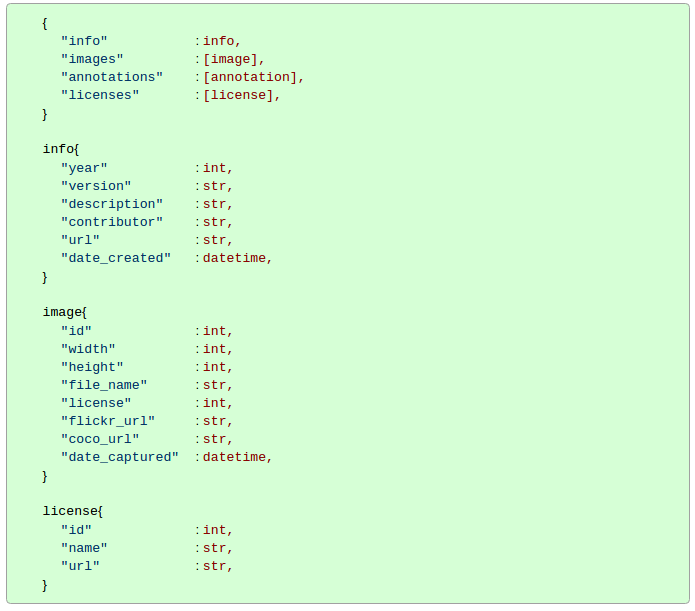
\includegraphics[width=0.8\textwidth]{figures/basic_structure_annotations.png}
		\caption{Estructura básica de anotaciones}
		\label{fig.basicStruc}
	\end{center}
\end{figure} 

\begin{figure}
	\begin{center}
		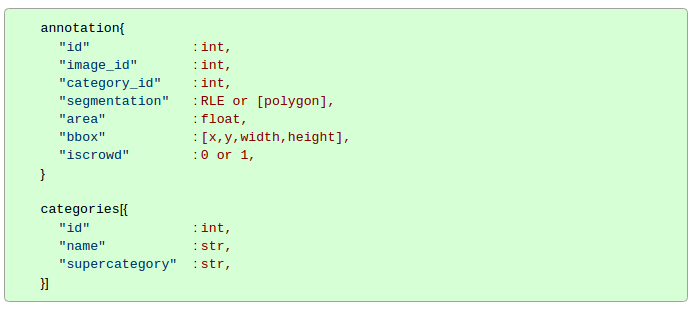
\includegraphics[width=0.8\textwidth]{figures/instancia_objetos.png}
		\caption{Estructura de instancias de objetos}
		\label{fig.objInst}
	\end{center}
\end{figure} 


